
\documentclass[11pt,letterpaper]{article}

% ---------------------------------------------------------
% Paquetes
% ---------------------------------------------------------

\usepackage[utf8]{inputenc}
\usepackage[T1]{fontenc}
\usepackage[spanish]{babel}
\usepackage{graphicx}
\usepackage{geometry}
\usepackage{amsmath}
\usepackage{amssymb}
\usepackage{listings}
\usepackage{xcolor}
\usepackage{float}
\usepackage{booktabs}
\usepackage{array}
\usepackage[hidelinks]{hyperref}

\geometry{letterpaper, margin=2.1cm}

% ---------------------------------------------------------
% Configuracion de codigo
% ---------------------------------------------------------

\lstset{
    language=Python,
    basicstyle=\ttfamily\footnotesize,
    keywordstyle=\color{blue},
    commentstyle=\color{gray},
    stringstyle=\color{red!60!black},
    numbers=left,
    numberstyle=\tiny,
    frame=single,
    breaklines=true,
    showstringspaces=false,
    columns=fullflexible,
    keepspaces=true
}

% ---------------------------------------------------------
% Datos
% ---------------------------------------------------------

\title{Taller 6: Espectro de Imágenes y Transformada Discreta de Fourier}

\author{
Camilo Eduardo Muñoz Albornoz\\
Procesamiento Digital de Imágenes\\
Universidad Tecnológica de Pereira
}

\date{}

\begin{document}

\maketitle

\begin{center}

\textbf{Código fuente en GitHub}\\[0.2cm]

\textbf{Carpeta del Taller 6: }
\href
{https://github.com/CamiloMunozAL/ProcDImagenes/tree/main/taller6}
{\textcolor{blue}{
\underline{
\texttt{github.com/CamiloMunozAL/ProcDImagenes/tree/main/taller6}
}
}}

\vspace{0.2cm}

\textbf{Cuaderno Python: }
\href
{https://github.com/CamiloMunozAL/ProcDImagenes/blob/main/taller6/taller6.ipynb}
{\textcolor{blue}{
\underline{\texttt{taller6.ipynb}}
}}

\end{center}

% =========================================================
\begin{abstract}

En este taller se estudió la representación de imágenes
digitales en el dominio de la frecuencia mediante la
Transformada Discreta de Fourier bidimensional (DFT 2D).

Se implementó una función con cuatro ciclos anidados
para calcular directamente los coeficientes de Fourier
de imágenes en escala de grises. Posteriormente, se
visualizaron sus espectros de magnitud mediante centrado
y escala logarítmica.

Finalmente, se implementó una segunda versión de la DFT
2D utilizando la propiedad de separabilidad, mediante
transformadas unidimensionales calculadas también con
ciclos.

Los algoritmos se probaron con cuatro imágenes sintéticas
de $64\times64$ píxeles: cuadrado, círculo, franjas
verticales e imagen uniforme. Los resultados se
verificaron numéricamente y se compararon los tiempos
de ejecución de ambos métodos.

\end{abstract}

% =========================================================
\section{Objetivos}

Los objetivos del taller fueron:

\begin{enumerate}

    \item Desarrollar una función basada en ciclos que
    permita realizar la Transformada Discreta de Fourier
    en 2D, aplicando el algoritmo a imágenes en escala
    de grises.

    \item Visualizar el espectro de las imágenes utilizando
    una escala logarítmica para facilitar la interpretación
    de sus componentes de frecuencia.

    \item Desarrollar una función basada en ciclos que
    realice la DFT en 2D utilizando la propiedad de
    separabilidad, y verificar sus resultados mediante
    una comparación con la implementación directa.

\end{enumerate}

% =========================================================
\section{Fundamentos teóricos}

\subsection{Dominio espacial y dominio de la frecuencia}

Una imagen digital en escala de grises puede representarse
como una matriz cuyos elementos corresponden a intensidades
de píxeles.

En el \textbf{dominio espacial}, cada valor corresponde
a una posición específica dentro de la imagen.

Por otro lado, en el \textbf{dominio de la frecuencia},
la información se representa mediante componentes que
describen patrones de variación de intensidad.

Las frecuencias espaciales permiten identificar qué tan
rápidamente cambian las intensidades entre los píxeles
de una imagen.

Las \textbf{frecuencias bajas} están relacionadas
con cambios graduales de intensidad y estructuras
amplias.

Las \textbf{frecuencias altas} están relacionadas
con cambios rápidos de intensidad, bordes y detalles
finos.

Por ejemplo, una imagen completamente uniforme no
presenta variaciones espaciales, mientras que una imagen
con franjas blancas y negras repetidas contiene
componentes de frecuencia relacionadas con la
periodicidad de las franjas.

\subsection{Transformada Discreta de Fourier 2D}

La Transformada Discreta de Fourier permite convertir
una imagen del dominio espacial al dominio de la
frecuencia.

Para una imagen $f(x,y)$ de $M$ filas y $N$ columnas,
la DFT 2D normalizada se define como:

\begin{equation}
F(u,v)=
\frac{1}{MN}
\sum_{x=0}^{M-1}
\sum_{y=0}^{N-1}
f(x,y)
e^{-i2\pi\left(
\frac{ux}{M}+\frac{vy}{N}
\right)}
\label{eq:dft2}
\end{equation}

Donde:

\begin{itemize}

    \item $f(x,y)$ representa la intensidad del
    píxel original.

    \item $M$ y $N$ representan las dimensiones
    de la imagen.

    \item $x$ y $y$ representan las posiciones
    espaciales de los píxeles.

    \item $u$ y $v$ representan los índices
    de frecuencia.

    \item $F(u,v)$ representa un coeficiente
    complejo de Fourier.

\end{itemize}

La exponencial compleja puede expresarse utilizando
la identidad de Euler:

\begin{equation}
e^{-i\theta}=
\cos(\theta)-i\sin(\theta)
\end{equation}

Esto explica por qué los coeficientes de Fourier
pueden tener una parte real y una parte imaginaria.

Una característica importante es que cada coeficiente
$F(u,v)$ se calcula considerando todos los píxeles
de la imagen.

Por esta razón, una implementación directa de la DFT
2D requiere cuatro ciclos anidados: dos para seleccionar
la frecuencia y dos para recorrer las intensidades
de la imagen.

\subsection{Componente continua o DC}

La componente continua corresponde a la frecuencia
cero de una imagen.

Cuando:

\[
u=0,\qquad v=0
\]

la exponencial de Fourier es igual a uno.

Por lo tanto:

\begin{equation}
F(0,0)=
\frac{1}{MN}
\sum_{x=0}^{M-1}
\sum_{y=0}^{N-1}
f(x,y)
\end{equation}

Con la normalización utilizada en este taller,
$F(0,0)$ es equivalente al promedio de intensidad
de todos los píxeles.

Por ejemplo, si una imagen uniforme tiene todos
sus píxeles con intensidad 128:

\[
F(0,0)=128
\]

Esta componente permite conocer el nivel promedio
de intensidad, pero no describe la forma o ubicación
de los objetos.

\subsection{Magnitud y fase}

Los coeficientes de Fourier son números complejos
que contienen información de magnitud y fase.

Para un número complejo:

\[
F(u,v)=a+ib
\]

su magnitud se calcula mediante:

\begin{equation}
|F(u,v)|=\sqrt{a^2+b^2}
\end{equation}

La magnitud permite identificar la contribución
de una componente de frecuencia.

La fase contiene información relacionada con
la organización espacial de las estructuras
presentes en la imagen.

Ambas son importantes para representar
y reconstruir correctamente una imagen
en el dominio espacial.

\subsection{Espectro de Fourier}

El espectro de Fourier es una representación
visual de las magnitudes de los coeficientes
de frecuencia de una imagen.

En la representación habitual, se reorganizan
los coeficientes para ubicar la frecuencia
cero en el centro del espectro.

De esta manera:

\begin{itemize}

    \item El centro corresponde a la frecuencia cero.

    \item Las regiones cercanas al centro contienen
    frecuencias bajas.

    \item Las regiones más alejadas del centro
    contienen frecuencias más altas.

    \item Los puntos más brillantes representan
    componentes de mayor magnitud dentro
    de la escala utilizada.

\end{itemize}

El espectro no representa directamente los
objetos de la imagen original, sino los
patrones de frecuencia que la componen.

\subsection{Escala logarítmica}

Los coeficientes de Fourier pueden presentar
magnitudes muy diferentes.

Si estas magnitudes se representan directamente,
los valores más grandes pueden dominar
la visualización y dificultar la identificación
de componentes más pequeñas.

Por esta razón, se utiliza una transformación
logarítmica:

\begin{equation}
S(u,v)=
\ln\left(1+|F_c(u,v)|\right)
\end{equation}

Donde $F_c(u,v)$ representa la transformada
con las frecuencias centradas.

En Python esta operación se realiza mediante:

\begin{lstlisting}
espectro = np.log1p(np.abs(centrada))
\end{lstlisting}

La función \texttt{np.abs()} obtiene la magnitud
de los coeficientes complejos.

La función \texttt{np.log1p()} calcula
el logaritmo natural de uno más cada magnitud.

Este procedimiento no genera nuevas frecuencias,
sino que facilita su visualización.

\subsection{Propiedad de separabilidad}

La DFT 2D tiene una propiedad importante llamada
\textbf{separabilidad}.

Esta propiedad permite calcular una transformada
bidimensional mediante dos transformaciones
unidimensionales sucesivas.

Esto es posible porque:

\begin{equation}
e^{-i2\pi\left(
\frac{ux}{M}+\frac{vy}{N}
\right)}
=
e^{-i2\pi\frac{ux}{M}}
\cdot
e^{-i2\pi\frac{vy}{N}}
\end{equation}

Por lo tanto, podemos aplicar primero una
transformada sobre las filas y después
una transformada sobre las columnas.

El resultado será equivalente al obtenido
mediante la DFT 2D directa.

Esta propiedad permite reducir considerablemente
la cantidad de operaciones necesarias.

Mientras la implementación directa requiere:

\[
O(M^2N^2)
\]

la implementación separable con DFT 1D
calculada mediante sumatorias requiere:

\[
O(MN^2+NM^2)
\]

% =========================================================
\section{Desarrollo y resultados}

\subsection{Preparación de las imágenes de prueba}

Para desarrollar los ejercicios se utilizaron cuatro
imágenes sintéticas de $64\times64$ píxeles.

Se escogieron imágenes sencillas para facilitar
la interpretación de sus espectros y evitar
los elevados tiempos de procesamiento
que produciría una fotografía grande.

Las imágenes utilizadas fueron:

\begin{itemize}

    \item Cuadrado blanco sobre fondo negro.

    \item Círculo blanco sobre fondo negro.

    \item Franjas verticales blancas y negras.

    \item Imagen uniforme de intensidad 128.

\end{itemize}

Las imágenes se generaron directamente con NumPy.

\begin{lstlisting}
import numpy as np
import matplotlib.pyplot as plt
import time

tamano = 64

# 1. Cuadrado blanco de 32x32
cuadrado = np.zeros(
    (tamano, tamano),
    dtype=np.float64
)

cuadrado[16:48, 16:48] = 255

# 2. Circulo blanco de radio 16
circulo = np.zeros(
    (tamano, tamano),
    dtype=np.float64
)

centro = tamano // 2
radio = 16

for i in range(tamano):
    for j in range(tamano):

        if (
            (i - centro)**2
            + (j - centro)**2
            <= radio**2
        ):
            circulo[i, j] = 255

# 3. Franjas verticales
franjas = np.zeros(
    (tamano, tamano),
    dtype=np.float64
)

for i in range(tamano):
    for j in range(tamano):

        if (j // 8) % 2 == 0:
            franjas[i, j] = 255

# 4. Imagen uniforme
uniforme = np.full(
    (tamano, tamano),
    128,
    dtype=np.float64
)

imagenes = [
    cuadrado,
    circulo,
    franjas,
    uniforme
]

titulos = [
    "Cuadrado",
    "Circulo",
    "Franjas verticales",
    "Imagen uniforme"
]
\end{lstlisting}

Las cuatro imágenes sintéticas generadas se muestran
en la Figura~\ref{fig:imagenes_sinteticas}.

\begin{figure}[H]
    \centering
    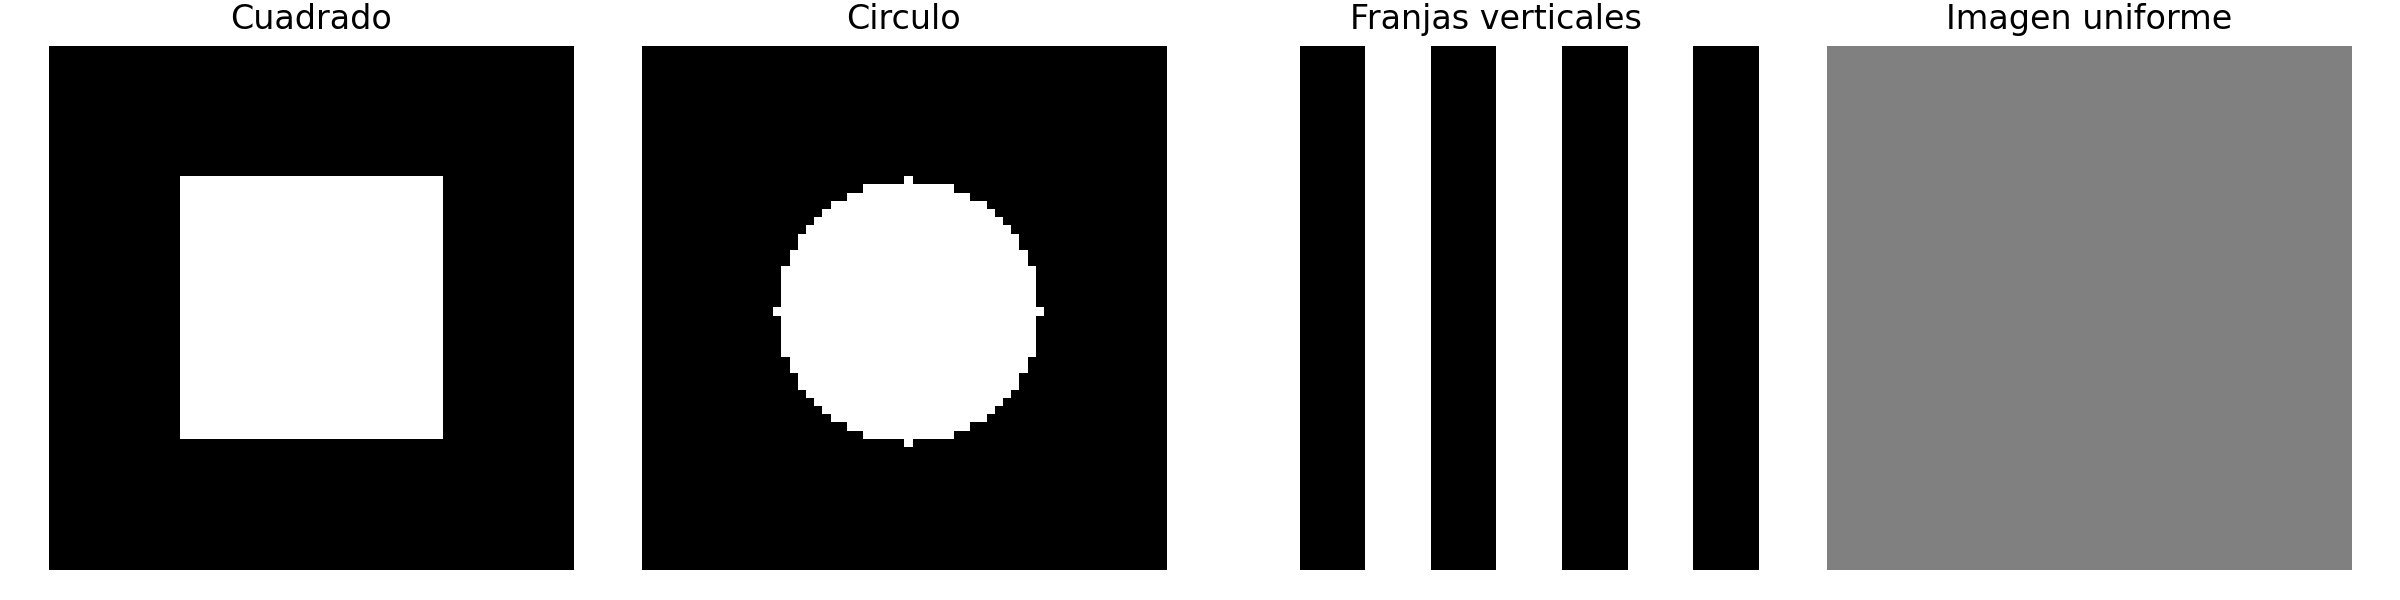
\includegraphics[width=0.95\textwidth]
    {../results/imagenes_sinteticas.png}
    \caption{
    Imágenes sintéticas utilizadas como entradas:
    cuadrado, círculo, franjas verticales e imagen uniforme.
    }
    \label{fig:imagenes_sinteticas}
\end{figure}

% =========================================================
\subsection{Punto 1: Implementación directa de la DFT 2D}

\subsubsection*{Objetivo}

Desarrollar una función basada en ciclos que permita
realizar la Transformada Discreta de Fourier en 2D,
aplicándola a imágenes en escala de grises.

\subsubsection*{Implementación}

Para este punto se desarrolló una función que
calcula directamente la DFT 2D utilizando
cuatro ciclos anidados.

Los dos primeros ciclos seleccionan la frecuencia
$(u,v)$ que se desea calcular.

Los dos ciclos interiores recorren todos los píxeles
de la imagen para calcular la contribución
de cada intensidad a dicha frecuencia.

La función implementada fue:

\begin{lstlisting}
def dft2d(imagen):

    # Dimensiones de la imagen
    # M = filas, N = columnas
    M, N = imagen.shape

    # Matriz compleja para almacenar la DFT
    resultado = np.zeros(
        (M, N),
        dtype=complex
    )

    # Recorrer cada frecuencia u y v
    for u in range(M):
        for v in range(N):

            suma = 0j

            # Recorrer todos los pixeles
            for x in range(M):
                for y in range(N):

                    # Calcular el angulo
                    angulo = -2 * np.pi * (
                        (u * x / M)
                        + (v * y / N)
                    )

                    # Exponencial compleja
                    exponencial = np.exp(
                        angulo * 1j
                    )

                    # Valor del pixel
                    pixel = imagen[x, y]

                    # Acumular la suma
                    suma += pixel * exponencial

            # Normalizar la DFT
            resultado[u, v] = suma / (M * N)

    return resultado
\end{lstlisting}

Se utilizó \texttt{dtype=complex} porque
los coeficientes de Fourier pueden tener
partes reales e imaginarias.

La variable \texttt{suma} se inicializó con
\texttt{0j}, que representa el número complejo cero.

En cada iteración se calcula el producto entre
la intensidad de un píxel y una exponencial compleja,
acumulando los resultados para obtener
el coeficiente correspondiente.

Finalmente, se divide entre $M\cdot N$,
siguiendo la normalización utilizada
en las diapositivas.

\subsubsection*{Aplicación a las cuatro imágenes}

Se aplicó la función a las cuatro imágenes
de $64\times64$ píxeles.

También se midió el tiempo de ejecución
mediante \texttt{time.perf\_counter()}.

El código utilizado fue:

\begin{lstlisting}
transformadas = []

for titulo, imagen_actual in zip(
    titulos,
    imagenes
):

    inicio = time.perf_counter()

    transformada = dft2d(
        imagen_actual
    )

    transformadas.append(
        transformada
    )

    tiempo = (
        time.perf_counter() - inicio
    )

    # Comparacion con NumPy
    referencia = (
        np.fft.fft2(imagen_actual)
        / imagen_actual.size
    )

    correcto = np.allclose(
        transformada,
        referencia,
        atol=1e-10
    )

    print(f"{titulo}:")
    print(f"  Tiempo: {tiempo:.2f} segundos")
    print(f"  Dimensiones: {transformada.shape}")
    print(f"  Coincide con NumPy: {correcto}")
    print()
\end{lstlisting}

La función \texttt{np.fft.fft2()} solamente
se utilizó como referencia para validar
la implementación manual.

Como NumPy no normaliza por defecto la
transformada directa, fue necesario dividir
su resultado entre el número de píxeles:

\begin{lstlisting}
np.fft.fft2(imagen_actual) / imagen_actual.size
\end{lstlisting}

Para comprobar la equivalencia numérica
se utilizó:

\begin{lstlisting}
np.allclose(
    transformada,
    referencia,
    atol=1e-10
)
\end{lstlisting}

Esta función permite comparar matrices
considerando pequeñas diferencias debidas
a la precisión numérica.

\subsubsection*{Resultados}

Los tiempos medidos fueron:

\begin{table}[H]
\centering
\caption{Resultados de la DFT 2D directa.}
\label{tab:directa}

\begin{tabular}{lccc}
\toprule
\textbf{Imagen} &
\textbf{Tiempo (s)} &
\textbf{Dimensiones} &
\textbf{Validación}\\
\midrule
Cuadrado & 16,80 & $64\times64$ & True\\
Círculo & 16,74 & $64\times64$ & True\\
Franjas verticales & 16,82 & $64\times64$ & True\\
Imagen uniforme & 16,85 & $64\times64$ & True\\
\bottomrule
\end{tabular}

\end{table}

\subsubsection*{Análisis de resultados}

Se implementó una función para calcular
la Transformada Discreta de Fourier en 2D
mediante cuatro ciclos anidados, utilizando
directamente su definición matemática.

Para comprobar su funcionamiento se utilizaron
cuatro imágenes sintéticas en escala de grises
de $64\times64$ píxeles: un cuadrado, un círculo,
franjas verticales y una imagen uniforme.

Los tiempos de ejecución estuvieron entre
16,74 y 16,85 segundos por imagen.

Estos tiempos fueron similares porque
el algoritmo recorre todos los píxeles
para calcular cada coeficiente de frecuencia,
independientemente del contenido de la imagen.

En una imagen de $64\times64$ se calculan
4096 coeficientes de frecuencia.

Para cada uno se recorren nuevamente
los 4096 píxeles originales.

Por tanto, el número de contribuciones es:

\[
64^4=16\,777\,216
\]

Posteriormente, se compararon las transformadas
calculadas manualmente con los resultados de
\texttt{np.fft.fft2()}, teniendo en cuenta
la normalización utilizada.

Las cuatro comparaciones devolvieron
\texttt{True}, lo que permitió verificar
que la implementación produce resultados
numéricamente equivalentes a los de NumPy.

En conclusión, se logró implementar y validar
la DFT 2D mediante ciclos, comprobando que
permite representar las imágenes del dominio
espacial en el dominio de la frecuencia.

También se observó que la implementación directa
requiere un tiempo de procesamiento considerable,
incluso con imágenes pequeñas.

% =========================================================
\subsection{Punto 2: Visualización del espectro logarítmico}

\subsubsection*{Objetivo}

Visualizar los espectros de las imágenes
utilizando escala logarítmica e interpretar
las componentes de frecuencia presentes
en cada una.

\subsubsection*{Implementación}

Para este punto se utilizaron las transformadas
obtenidas anteriormente.

No fue necesario volver a calcular
la DFT 2D.

Primero se utilizó:

\begin{lstlisting}
np.fft.fftshift(transformada)
\end{lstlisting}

para colocar la frecuencia cero en el centro.

Posteriormente:

\begin{lstlisting}
np.abs(centrada)
\end{lstlisting}

para obtener las magnitudes de los coeficientes.

Finalmente:

\begin{lstlisting}
np.log1p(np.abs(centrada))
\end{lstlisting}

para facilitar la visualización del espectro
mediante escala logarítmica.

El código completo fue:

\begin{lstlisting}
fig, axs = plt.subplots(
    4, 2,
    figsize=(10, 16)
)

for i, (
    imagen_actual,
    transformada,
    titulo
) in enumerate(
    zip(imagenes, transformadas, titulos)
):

    # Centrar la transformada
    centrada = np.fft.fftshift(
        transformada
    )

    # Espectro logaritmico
    espectro = np.log1p(
        np.abs(centrada)
    )

    # Imagen original
    axs[i, 0].imshow(
        imagen_actual,
        cmap="gray",
        vmin=0,
        vmax=255,
        interpolation="nearest"
    )

    axs[i, 0].set_title(titulo)
    axs[i, 0].axis("off")

    # Espectro de Fourier
    axs[i, 1].imshow(
        espectro,
        cmap="gray",
        interpolation="nearest"
    )

    axs[i, 1].set_title(
        f"Espectro - {titulo}"
    )

    axs[i, 1].axis("off")

plt.tight_layout()

plt.savefig(
    "results/espectros_dft.png",
    dpi=150
)

plt.show()
\end{lstlisting}

Los resultados se observan en la
Figura~\ref{fig:espectros}.

\begin{figure}[H]
    \centering

    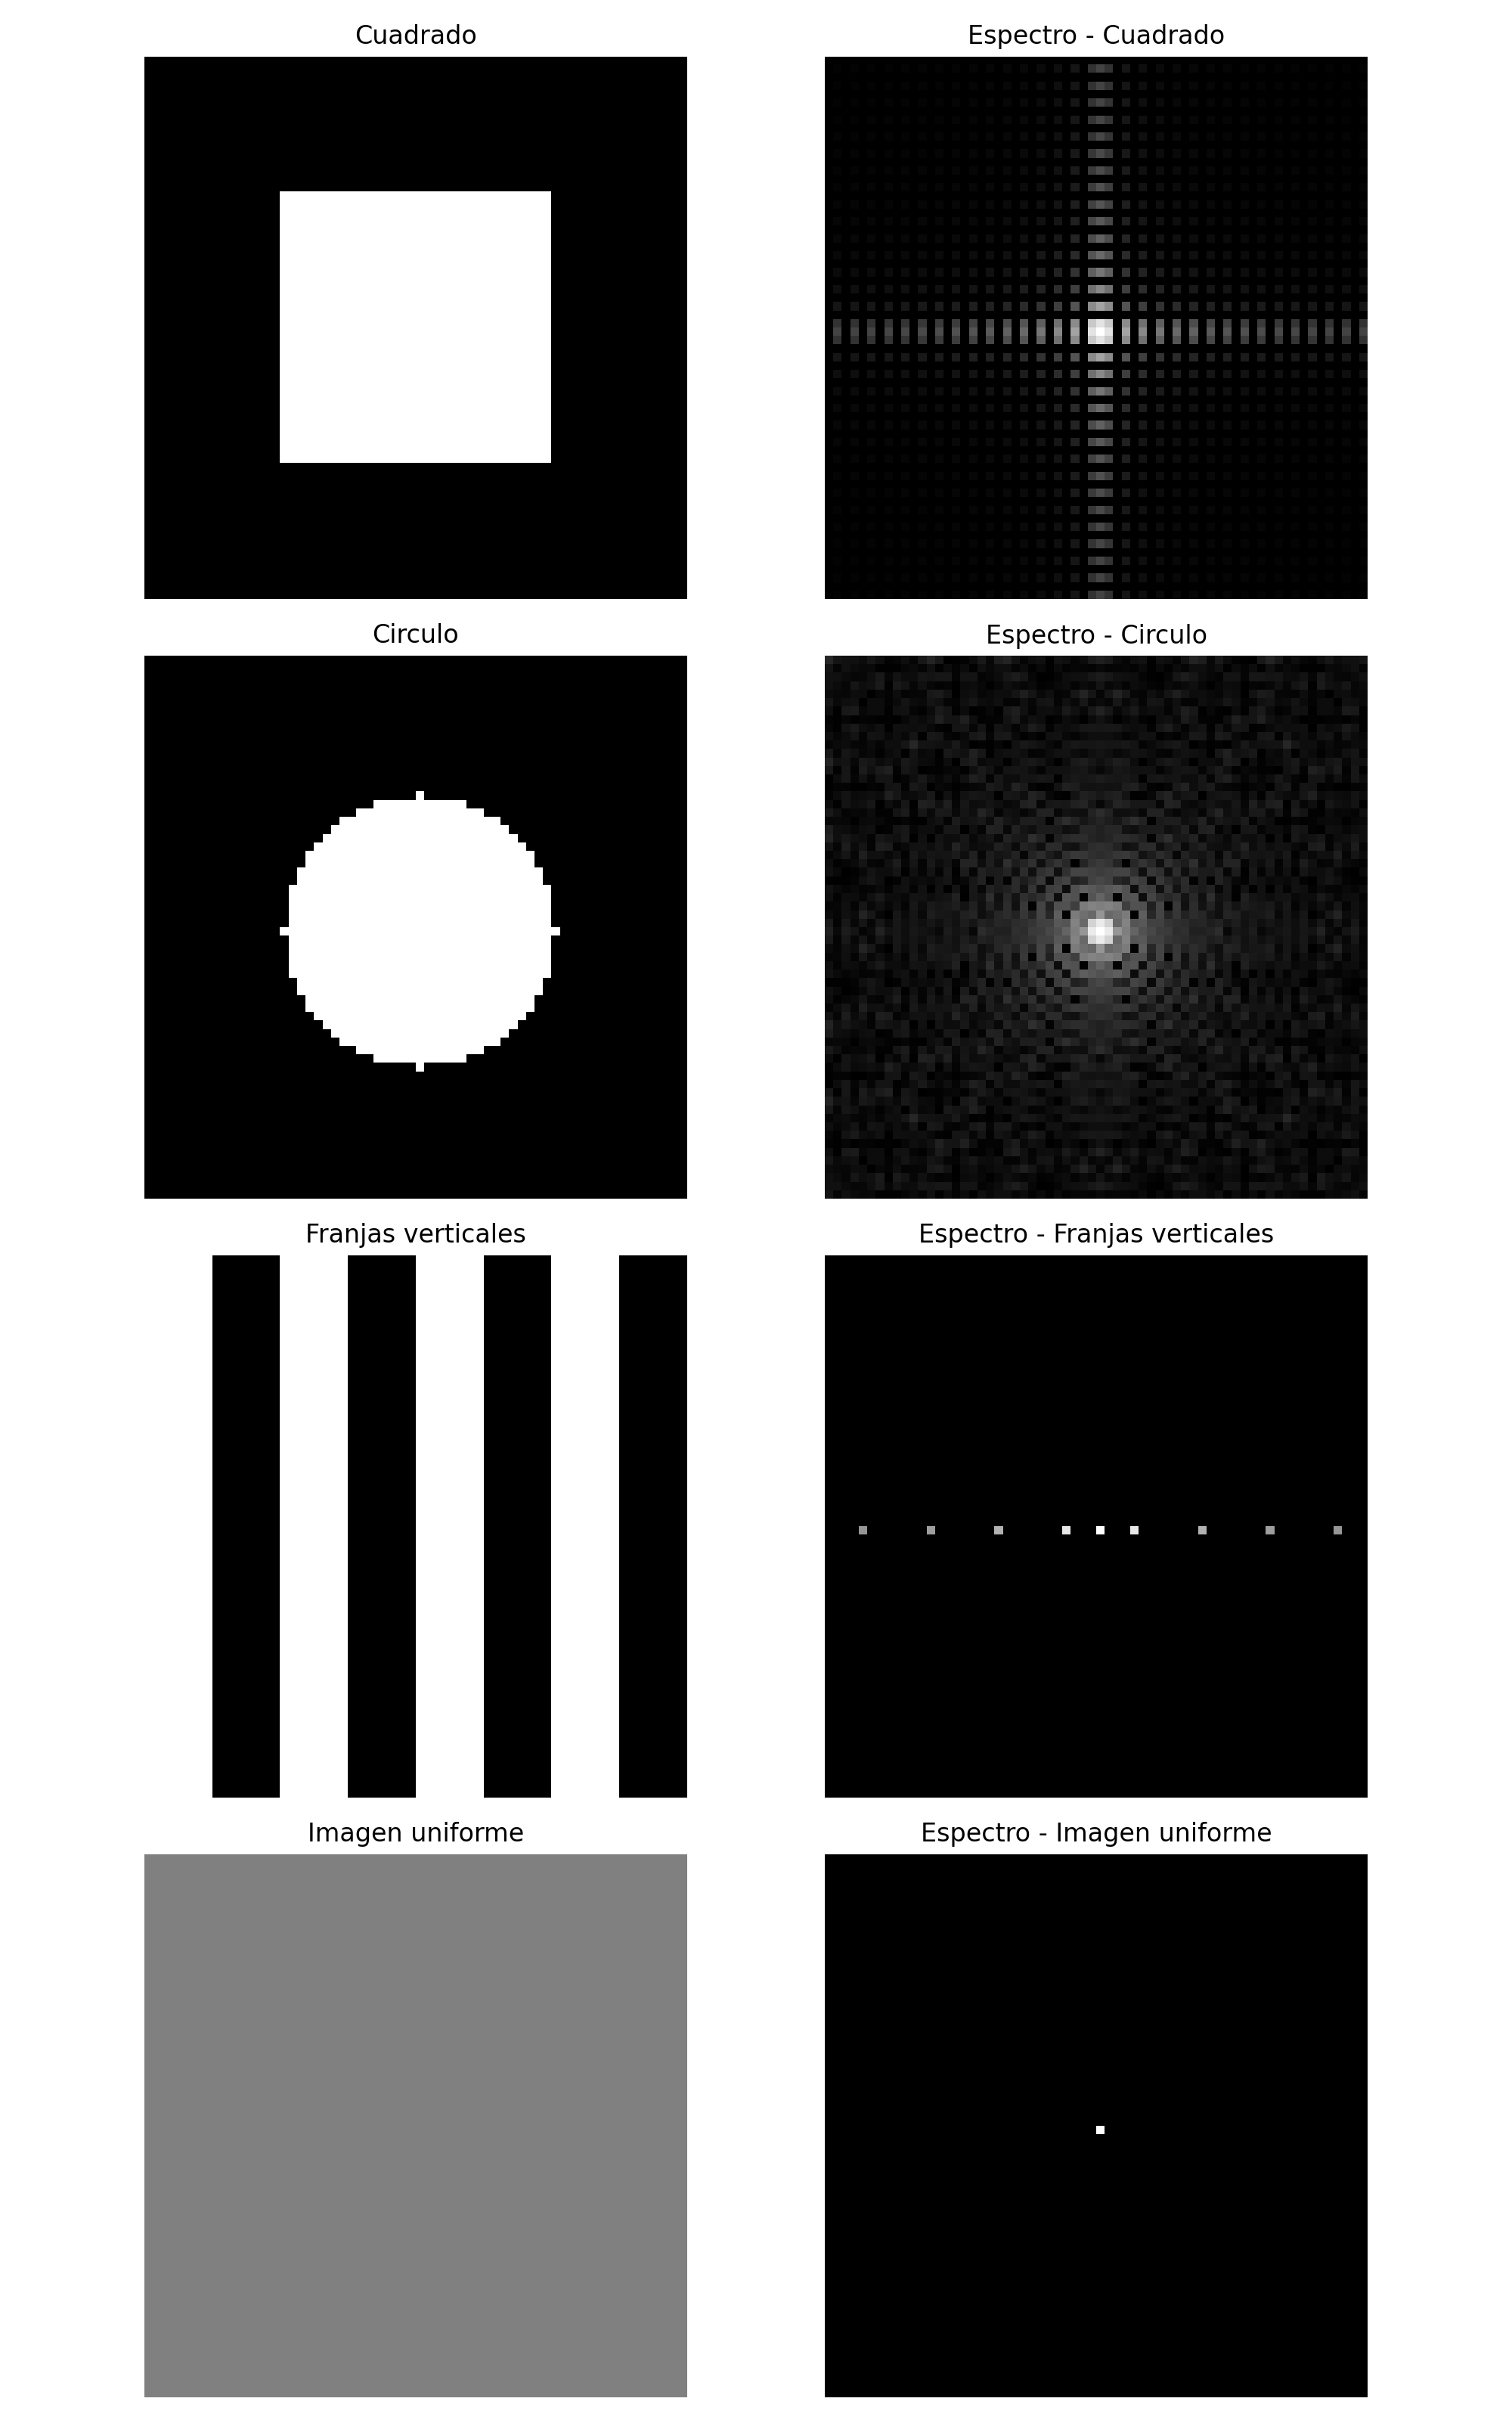
\includegraphics[width=0.90\textwidth]
    {../results/espectros_dft.png}

    \caption{
    Imágenes originales de $64\times64$
    y sus correspondientes espectros de Fourier
    centrados y representados en escala logarítmica.
    }

    \label{fig:espectros}
\end{figure}

\subsubsection*{Análisis de resultados}

Se visualizaron los espectros de Fourier
de las cuatro imágenes utilizando la magnitud
de la transformada y una escala logarítmica.

También se centraron los espectros
para ubicar la frecuencia cero
en el centro de cada representación.

\paragraph{Cuadrado}

En la imagen del cuadrado, el espectro
presenta una estructura en forma de cruz
con múltiples puntos brillantes y oscuros.

Esto se relaciona con sus bordes horizontales
y verticales.

La presencia de diferentes componentes
se debe a los cambios bruscos de intensidad
entre el cuadrado blanco y el fondo negro.

Los puntos observados representan máximos
y mínimos de las magnitudes de frecuencia.

\paragraph{Círculo}

En el círculo se observa una distribución
aproximadamente circular, con anillos
alrededor del centro.

Esto ocurre debido a la simetría radial
de la figura, que también se manifiesta
en su espectro de frecuencias.

Los anillos representan variaciones
en las magnitudes de las componentes
de frecuencia.

Debido a que el círculo se representa
mediante píxeles, sus bordes son escalonados
y los anillos no son perfectamente uniformes.

\paragraph{Franjas verticales}

En la imagen de franjas verticales aparecen
puntos brillantes distribuidos sobre
el eje horizontal del espectro.

Esto sucede porque los cambios de intensidad
se presentan periódicamente de izquierda
a derecha.

Las distintas componentes corresponden
a las frecuencias que forman ese patrón
repetitivo.

También aparecen componentes adicionales
debido a las transiciones bruscas
entre blanco y negro.

\paragraph{Imagen uniforme}

Finalmente, la imagen uniforme presenta
únicamente un punto brillante en el centro
del espectro.

Esto ocurre porque todos los píxeles
tienen la misma intensidad y no existen
variaciones espaciales.

El punto central representa la componente
continua o frecuencia cero.

Como la intensidad de todos los píxeles
es 128:

\[
F(0,0)=128
\]

Las demás componentes tienen magnitudes
prácticamente iguales a cero.

\subsubsection*{Conclusión del punto}

Los espectros obtenidos muestran que
la Transformada de Fourier permite identificar
características de las imágenes mediante
sus componentes de frecuencia.

Las formas, los bordes, la orientación
y la repetición de patrones producen
distribuciones diferentes en el espectro.

Por tanto, este procedimiento permite
analizar una imagen desde una representación
distinta al dominio espacial.

% =========================================================
\subsection{Punto 3: DFT 2D mediante separabilidad}

\subsubsection*{Objetivo}

Desarrollar una función basada en ciclos
que realice la DFT en 2D utilizando
la propiedad de separabilidad.

Comprobar que los resultados coincidan
con la implementación directa
y comparar los tiempos de ejecución.

\subsubsection*{Implementación de la DFT 1D}

La propiedad de separabilidad permite
obtener una DFT 2D mediante transformadas
unidimensionales sucesivas.

Por esta razón, primero se desarrolló
una función para calcular la DFT 1D
utilizando dos ciclos anidados.

La expresión matemática es:

\begin{equation}
F(k)=
\frac{1}{N}
\sum_{n=0}^{N-1}
f(n)e^{-i2\pi kn/N}
\end{equation}

La función desarrollada fue:

\begin{lstlisting}
def dft1d(vector):

    N = len(vector)

    resultado = np.zeros(
        N,
        dtype=complex
    )

    for k in range(N):

        suma = 0j

        for n in range(N):

            angulo = (
                -2 * np.pi * k * n / N
            )

            exponencial = np.exp(
                1j * angulo
            )

            suma += (
                vector[n] * exponencial
            )

        resultado[k] = suma / N

    return resultado
\end{lstlisting}

Esta función recibe un vector y calcula
sus coeficientes de frecuencia.

El primer ciclo recorre las frecuencias
y el segundo recorre los elementos
del vector original.

En este caso no se utilizó
\texttt{np.fft.fft()}, ya que se implementó
manualmente la DFT mediante ciclos.

\subsubsection*{Implementación de la DFT 2D separable}

Posteriormente, se desarrolló una función
que aplica la DFT 1D sobre cada fila
y después sobre cada columna.

\begin{lstlisting}
def dft2d_separable(imagen):

    M, N = imagen.shape

    # Primera etapa: DFT sobre las filas
    transformada_filas = np.zeros(
        (M, N),
        dtype=complex
    )

    for fila in range(M):

        transformada_filas[fila, :] = dft1d(
            imagen[fila, :]
        )

    # Segunda etapa: DFT sobre las columnas
    resultado = np.zeros(
        (M, N),
        dtype=complex
    )

    for columna in range(N):

        resultado[:, columna] = dft1d(
            transformada_filas[:, columna]
        )

    return resultado
\end{lstlisting}

En la primera etapa se calcula la DFT
de cada fila de la imagen.

En la segunda etapa se calcula la DFT
de cada columna de la matriz intermedia.

La función \texttt{dft1d()} ya realiza
la normalización de cada transformación
unidimensional.

Primero se divide entre $N$
y después entre $M$.

Por tanto, la normalización total es:

\[
\frac{1}{N}\cdot\frac{1}{M}
=
\frac{1}{MN}
\]

Esto coincide con la normalización
utilizada en el punto 1.

\subsubsection*{Aplicación y comparación}

Se aplicó el algoritmo separable
a las mismas cuatro imágenes.

También se compararon sus resultados
con las transformadas obtenidas
mediante el método directo.

El código utilizado fue:

\begin{lstlisting}
transformadas_separables = []

for (
    titulo,
    imagen_actual,
    transformada_directa
) in zip(
    titulos,
    imagenes,
    transformadas
):

    inicio = time.perf_counter()

    resultado = dft2d_separable(
        imagen_actual
    )

    tiempo = (
        time.perf_counter() - inicio
    )

    transformadas_separables.append(
        resultado
    )

    correcto = np.allclose(
        resultado,
        transformada_directa,
        atol=1e-10
    )

    diferencia = np.max(
        np.abs(
            resultado - transformada_directa
        )
    )

    print(f"{titulo}:")
    print(f"  Tiempo: {tiempo:.4f} segundos")
    print(f"  Coincide con DFT directa: {correcto}")
    print(f"  Diferencia maxima: {diferencia:.2e}")
    print()
\end{lstlisting}

\subsubsection*{Resultados}

Los valores obtenidos fueron:

\begin{table}[H]
\centering
\caption{Comparación entre la DFT directa y separable.}
\label{tab:comparacion}

\small

\begin{tabular}{lccc}
\toprule
\textbf{Imagen} &
\textbf{Directa (s)} &
\textbf{Separable (s)} &
\textbf{Aceleración}\\
\midrule
Cuadrado & 16,80 & 0,4783 & $35,1\times$\\
Círculo & 16,74 & 0,4827 & $34,7\times$\\
Franjas & 16,82 & 0,5200 & $32,3\times$\\
Uniforme & 16,85 & 0,4889 & $34,5\times$\\
\bottomrule
\end{tabular}

\end{table}

Todas las comparaciones devolvieron
\texttt{True}.

Las diferencias máximas entre ambos métodos
fueron:

\begin{table}[H]
\centering
\caption{Diferencias numéricas entre las transformadas.}
\label{tab:diferencias}

\begin{tabular}{lc}
\toprule
\textbf{Imagen} & \textbf{Diferencia máxima}\\
\midrule
Cuadrado & $6,43\times10^{-13}$\\
Círculo & $5,42\times10^{-13}$\\
Franjas verticales & $6,38\times10^{-13}$\\
Imagen uniforme & $6,04\times10^{-13}$\\
\bottomrule
\end{tabular}

\end{table}

\subsubsection*{Análisis de resultados}

Se implementó la Transformada Discreta de Fourier
en 2D utilizando la propiedad de separabilidad.

Para ello, se desarrolló una función que calcula
manualmente la DFT en una dimensión mediante ciclos,
y posteriormente se aplicó sobre las filas
y columnas de cada imagen.

El algoritmo se probó con las cuatro imágenes
de $64\times64$ píxeles utilizadas anteriormente.

Los tiempos de ejecución estuvieron entre
0,4783 y 0,5200 segundos, valores considerablemente
inferiores a los obtenidos con la implementación
directa, que tardó aproximadamente 17 segundos
por imagen.

Al comparar ambos métodos, se observó una mejora
de velocidad de alrededor de 34 veces.

Esto sucede porque la separabilidad permite
calcular la transformada mediante dos etapas
unidimensionales, reduciendo la cantidad
de operaciones necesarias.

En una imagen de $64\times64$,
la implementación directa requiere:

\[
64^4=16\,777\,216
\]

contribuciones.

Mientras que la implementación separable
requiere:

\[
2\cdot64^3=524\,288
\]

contribuciones.

Por tanto, el algoritmo separable realiza
32 veces menos contribuciones
que el método directo.

Además, las comparaciones entre ambas
implementaciones devolvieron \texttt{True}
en los cuatro casos.

Las diferencias máximas fueron del orden
de $10^{-13}$.

Estas diferencias se deben a la precisión
numérica de los cálculos y no representan
modificaciones significativas en los resultados.

Es importante aclarar que la mejora observada
proviene de la propiedad de separabilidad,
ya que las transformadas unidimensionales
también fueron implementadas manualmente.

No se utilizó la FFT optimizada de NumPy
para efectuar el cálculo principal.

En conclusión, la propiedad de separabilidad
permitió calcular la misma DFT 2D de manera
mucho más eficiente, conservando resultados
numéricamente equivalentes.

% =========================================================
\section{Análisis general}

El desarrollo del taller permitió comprender
cómo una imagen digital puede analizarse
desde el dominio espacial y también
desde el dominio de la frecuencia.

En el primer ejercicio se comprobó que
la DFT 2D puede calcularse directamente
mediante su definición matemática,
utilizando cuatro ciclos anidados.

La implementación permitió identificar
que cada coeficiente de frecuencia
se obtiene considerando todos los píxeles
de la imagen original.

Posteriormente, la visualización de los
espectros permitió relacionar las estructuras
espaciales de diferentes imágenes
con sus componentes de frecuencia.

En el cuadrado se observó una estructura
espectral asociada con sus bordes
horizontales y verticales.

En el círculo apareció una distribución
aproximadamente radial, mientras que
las franjas verticales produjeron
componentes concentradas sobre
el eje horizontal del espectro.

Por su parte, la imagen uniforme
presentó únicamente la componente
continua debido a la ausencia de
variaciones espaciales de intensidad.

La escala logarítmica permitió distinguir
componentes de frecuencia que habrían
resultado difíciles de observar debido
a las grandes diferencias de magnitud.

Finalmente, la implementación mediante
separabilidad mostró que dos procedimientos
matemáticamente equivalentes pueden presentar
costos computacionales muy diferentes.

Mientras la DFT directa tardó en promedio
16,80 segundos, la implementación separable
redujo este tiempo a aproximadamente
0,49 segundos por imagen.

Además, los resultados fueron equivalentes
dentro de los límites de precisión numérica.

Esto permitió comprobar que las propiedades
matemáticas de un algoritmo pueden aprovecharse
para mejorar considerablemente su eficiencia.

% =========================================================
\section{Conclusiones}

Se logró implementar la Transformada Discreta
de Fourier bidimensional mediante cuatro ciclos
anidados, utilizando directamente su expresión
matemática.

Las cuatro imágenes de prueba produjeron
resultados equivalentes a los de NumPy,
teniendo en cuenta la normalización aplicada.

La visualización de los espectros centrados
en escala logarítmica permitió observar
que las diferentes formas, bordes
y patrones repetitivos generan
distribuciones de frecuencia distintas.

También se comprobó que una imagen uniforme
presenta únicamente la componente
de frecuencia cero, relacionada con
el promedio de intensidad.

La propiedad de separabilidad permitió
implementar la DFT 2D mediante dos etapas
de transformadas unidimensionales calculadas
manualmente.

Este procedimiento redujo el tiempo promedio
de aproximadamente 16,80 a 0,49 segundos
por imagen de $64\times64$ píxeles.

Las diferencias máximas del orden de
$10^{-13}$ demostraron que los dos
procedimientos producen resultados
numéricamente equivalentes.

En conjunto, el taller permitió comprender
la relación entre
dominio espacial, frecuencia espacial,
Transformada Discreta de Fourier,
espectro de magnitud, componente continua
y separabilidad.

Estos conceptos son fundamentales
para técnicas posteriores de análisis
y filtrado de imágenes en el dominio
de la frecuencia.

\end{document}
